% Runtime results
\section{Performance of EMS-GT with speedup techniques}
Every runtime evaluation using these speedup techniques was run using Intel Xeon, 2.10 Ghz machine. The performance of each algorithm was averaged over 20 synthetic datasets for each $(l, d)$-challenge instance where $l \leq 17$. This section shows the runtime performance of EMS-GT with different combinations of speedup techniques introduced in this study. The version of EMS-GT that yielded the fastest runtime performance was used in the proposed EMS-GT2 algorithm. Overall, these speedup techniques improved the runtime performance of EMS-GT algorithm with at least 12.77\%, 18.13\%, 2.15\%, 5.03\% and 4.23\% for (9, 2), (11, 3), (13, 4), (15, 5) and (17, 6) challenge instances respectively. 


% -------------------------------------------------------------------------------------------------

	\subsection{Evaluation of block boolean flag (BBF) technique}
	% Explanation
	Table \ref{tbl:ems-gt-bf-speedup} shows the runtime performance of block boolean flag technique with its corresponding runtime reductions from the original EMS-GT.

	% Show table
	\begin{table}[h] %speedup_blockmasking
	\renewcommand{\arraystretch}{1.3}
	\centering
	\begin{tabular}{|c|c|c|c|}
	\hline 
	\bfseries\boldmath $(l,d)$ & 
	\bfseries\boldmath EMS-GT & 
	\bfseries\boldmath EMS-GT with BBF & 
	\bfseries \% speedup\\
	\hline
	(9, 2) & 0.0468 s &		0.049 s &	-\\
	(11, 3) & 0.168 s &		0.172 s &	-\\
	(13, 4) & 1.180 s &		1.107 s &	6.21 \%\\
	(15, 5) & 12.767 s &	11.937 s &	6.51 \%\\
	(17, 6) & 143.215 s &	131.776 s &	7.99 \%\\
	\hline\end{tabular}
	
	\caption{EMS-GT with block boolean flags strategy.}
	\label{tbl:ems-gt-bf-speedup}
\end{table}




	% Short analysis
	The block boolean flags technique is efficient when there are significant amount of empty blocks in the candidate motif array. Using this technique, the generation of $d$-neighborhood can focus on those blocks with remaining candidate motifs. 

	Choosing the value for the parameter $n'$ plays a valuable role in this speedup technique. The more sequences processed during the Generation phase the smaller the size of the candidate motifs become and thus the number of empty blocks increases. As we process more sequence in the Generate phase, using the block boolean flags technique, the runtime in generating the $d$-neighborhood of a sequence decreases. Figure \ref{fig:bf-per-sequence-runtime} shows the average runtime in generating the $d$-neighborhood of a sequence per sequence number in (17, 6) problem instance. In evaluating the block boolean flags technique we use $n'=10$, which is the optimum value used also in the previous studies.

	\begin{figure}[h]
	\centering
	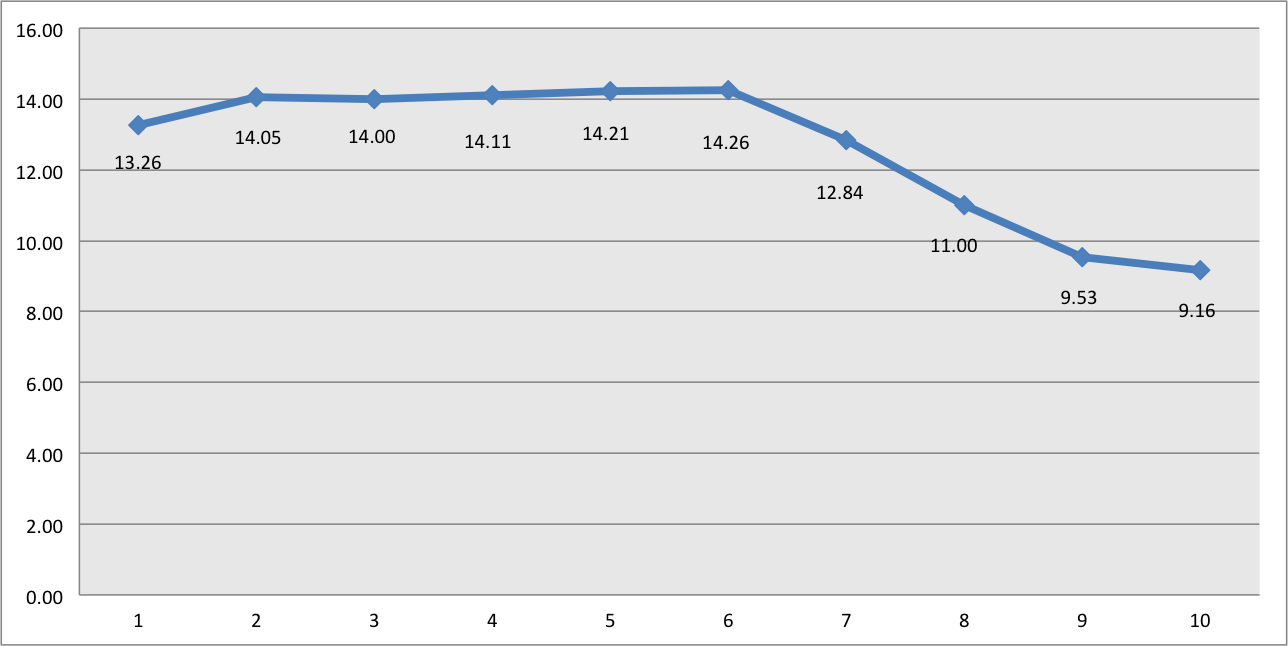
\includegraphics[width=4.5in]{contents/00_images/bf-sequence-runtime}
	\caption{Runtime (s) of $d$-neighborhood generation of sequence for all sequence in Generation Phase using (17, 6) problem instance.}
	\label{fig:bf-per-sequence-runtime}
\end{figure} 

	Additionally, we incorporated the improved hamming distance computation technique with block boolean flags technique resulting into faster runtime performance, which is shown in Table \ref{tbl:ems-gt-bf-hd-speedup}.

	\begin{table}[h] %speedup_blockmasking
	\renewcommand{\arraystretch}{1.3}
	\centering
	\begin{tabular}{|c|c|c|c|}
	\hline 
	\bfseries\boldmath $(l,d)$ & 
	\bfseries\boldmath EMS-GT & 
	\bfseries\boldmath EMS-GT with BBF and IHD & 
	\bfseries \% speedup\\
	\hline
	(9, 2) & 0.0468 s &		0.035 s 	&	25.00 \%\\
	(11, 3) & 0.168 s &		0.115 s 	&	31.91 \%\\
	(13, 4) & 1.180 s &		0.930 s 	&	21.27 \%\\
	(15, 5) & 12.767 s &	11.532 s  	&	9.68 \%\\
	(17, 6) & 143.215 s &	130.841 s 	&	8.64 \%\\
	\hline\end{tabular}
	
	\caption{EMS-GT with BBF strategy and improved hamming distance computation.}
	\label{tbl:ems-gt-bf-speedup}
\end{table}




% -------------------------------------------------------------------------------------------------

	\subsection{Evaluation of fast candidate motif elimination (FCE) technique}
	Runtime performance of fast candidate motif elimination technique is shown in Table \ref{tbl:ems-gt-fce-speedup}. Fast candidate motif elimination is used in the Test phase of the algorithm. This technique is efficient if there are a significant number of candidate motifs left in a block, unlike the block boolean flags technique that is efficient when there are numerous empty blocks in the candidate motifs array. This technique uses different values for $n'$ which are 10, 10, 9, 8 and 7 for the mentioned $(l, d)$ challenge instances respectively. 

	\begin{table}[h] %speedup_blockmasking
	\renewcommand{\arraystretch}{1.3}
	\centering
	\begin{tabular}{|c|c|c|c|}
	\hline 
	\bfseries\boldmath $(l,d)$ & 
	\bfseries\boldmath EMS-GT & 
	\bfseries\boldmath EMS-GT with FCE & 
	\bfseries \% speedup\\
	\hline
	(9, 2) & 0.0468 s &		0.051 s 	&	-\\
	(11, 3) & 0.168 s &		0.172 s 	&	-\\
	(13, 4) & 1.180 s &		1.340 s 	&	-\\
	(15, 5) & 12.767 s &	13.362 s  	&	-\\
	(17, 6) & 143.215 s &	135.799 s 	&	5.17 \%\\
	\hline\end{tabular}
	
	\caption{Runtime comparison of EMS-GT and EMS-GT with fast candidate motif elimination.}
	\label{tbl:ems-gt-fce-speedup}
\end{table}




	EMS-GT with fast candidate motif elimination technique alone only improved the runtime in (13, 4) and (17, 6) only by 2.15\% and 4.23\% respectively, but with the improved hamming distance computation, the runtime performance has greatly increased in all of the challenge instances used in the experimentations. The Test phase uses the hamming distance computation heavily and choosing the right sequence to start the Test phase greatly affects the runtime of the algorithm with these speedup techniques. Table \ref{tbl:ems-gt-fce-hd-speedup} shows the runtime performance of EMS-GT with fast candidate motif elimination technique and the improved hamming distance computation.

	\begin{table}[h] %speedup_blockmasking
	\renewcommand{\arraystretch}{1.3}
	\centering
	\begin{tabular}{|c|c|c|c|}
	\hline 
	\bfseries\boldmath $(l,d)$ & 
	\bfseries\boldmath EMS-GT & 
	\bfseries\boldmath EMS-GT with FCE and IHD & 
	\bfseries \% speedup\\
	\hline
	(9, 2) & 0.0468 s &		0.038 s 	&	18.33 \%\\
	(11, 3) & 0.168 s &		0.126 s 	&	25.46 \%\\
	(13, 4) & 1.180 s &		0.946 s 	&	19.88 \%\\
	(15, 5) & 12.767 s &	10.876 s  	&	14.82 \%\\
	(17, 6) & 143.215 s &	111.660 s 	&	22.03 \%\\
	\hline\end{tabular}
	
	\caption{Runtime comparison of EMS-GT and EMS-GT with fast candidate motif elimination and improved hamming distance computation.}
	\label{tbl:ems-gt-fce-hd-speedup}
\end{table}




	Finally, Table \ref{tbl:ems-gt-all-speedup} shows the runtime evaluation of EMS-GT with all of the speedup techniques having $n'$ values used in the fast candidate motif elimination experiments. For all the $(l, d)$ challenge instances used except (17, 6), EMS-GT with fast candidate motif elimination and improved hamming distance computation is still faster than EMS-GT with all speedup techniques. EMS-GT with all speedup techniques failed to compensate for the computational overhead it has introduced in the block boolean flags technique. Given this result, we used the fast candidate motif elimination and improved hamming distance computation only in the proposed EMS-GT2 algorithm.

	\begin{table}[h] %speedup_blockmasking
	\renewcommand{\arraystretch}{1.3}
	\centering
	\begin{tabular}{|c|c|c|c|}
	\hline 
	\bfseries\boldmath $(l,d)$ & 
	\bfseries\boldmath EMS-GT & 
	\bfseries\boldmath EMS-GT with FCE, BFF and IHD & 
	\bfseries \% speedup\\
	\hline
	(9, 2) & 0.0468 s &		0.040 s 	&	15.0 \%\\
	(11, 3) & 0.168 s &		0.134 s 	&	20.37 \%\\
	(13, 4) & 1.180 s &		1.112 s 	&	5.88 \%\\
	(15, 5) & 12.767 s &	11.252 s  	&	11.87 \%\\
	(17, 6) & 143.215 s &	111.634 s 	&	22.05 \%\\
	\hline\end{tabular}
	
	\caption{Runtime comparison of EMS-GT and EMS-GT with all speedup techniques.}
	\label{tbl:ems-gt-all-speedup}
\end{table}




% -------------------------------------------------------------------------------------------------


\section{Runtime performance comparison of EMS-GT2, EMS-GT and qPMS9}
The EMS-GT2, EMS-GT and qPMS9 were evaluated in terms of actual runtime on an Intel Xeon, 2.10 Ghz machine. The performance of each algorithm was averaged over synthetic datasets for each $(l, d)$-challenge instance where $l \leq 17$. Table \ref{tbl:final-results-ems} shows the runtime results between EMS-GT2 vs EMS-GT, while Table \ref{tbl:final-results} shows the runtime results between EMS-GT2 vs the algorithm qPMS9.


\begin{table}[h] %speedup_blockmasking
	\renewcommand{\arraystretch}{1.3}
	\centering
	\begin{tabular}{|c|c|c|c|}
	\hline 
	\bfseries\boldmath $(l,d)$ & 
	\bfseries EMS-GT & 
	\bfseries\boldmath EMS-GT2  & 
	\bfseries \% speedup\\
	\hline
	 (9,2) 	&  0.047 s &    0.038 s &    18.33 \%\\
	(11,3) &   0.168 s &    0.126 s &    25.46 \%\\
	(13,4) &   1.181 s &    0.946 s &   19.88 \%\\
	(15,5) &  12.768 s &   10.876 s &   14.81 \%\\
	(17,6) & 143.215 s &  111.660 s &   22.03 \%\\
	\hline\end{tabular}
	
	\caption{EMS-GT and EMS-GT2 runtime evaluation.}
	\label{tbl:final-results-ems}
\end{table}


% Explanation for Table final-results-ems
The additional speedup techniques become more effective as the $l$ value in the $(l, d)$-instance grows. For every $(l, d)$-challenge instances mentioned, EMS-GT2 has improved the runtime over the EMS-GT for at least 14.8\%. 

\begin{table}[h] %speedup_blockmasking
	\renewcommand{\arraystretch}{1.3}
	\centering
	\begin{tabular}{|c|c|c|c|}
	\hline 
	\bfseries\boldmath $(l,d)$ & 
	\bfseries qPMS9 & 
	\bfseries\boldmath EMS-GT2 & 
	\bfseries \% speedup\\
	\hline
	 (9,2) &   0.647 s &    0.039 s &   93.97 \%\\
	(11,3) &   1.276 s &    0.140 s &   89.02 \%\\
	(13,4) &   4.269 s &    0.758 s &   82.24 \%\\
	(15,5) &  24.737 s &   10.565 s &   57.29 \%\\
	(17,6) & 118.226 s &  112.311 s &   5.00 \%\\
	\hline\end{tabular}
	
	\caption{EMS-GT2 and qPMS9 runtime evaluation.}
	\label{tbl:final-results}
\end{table}




% Explanation for Table final-results
Previous implementations of EMS-GT failed to beat qPMS9 in $(17, 6)$-challenge instance. The proposed EMS-GT2 not only produces improved runtimes but also outperforms the qPMS9 in all of the $(l, d)$-challenge instances where $l \leq 17$. The efficiency of qPMS9 algorithm improves as the $l$ value increases, due to the fewer $l$-mer tuple combinations to consider. The performance of EMS-GT improves as $l$ value decreases, since there are fewer candidate motifs to consider. This is one reason why the previous implementation of EMS-GT was unsuccessful in beating qPMS9 in $(17, 6)$-challenge instance. The EMS-GT maintains a parameter $n'$ that directly affects the number of candidate motifs left to process in the Test phase. Fixing the value of $n'$ for all challenge instances fails to maximize the efficiency of the additional speedup techniques used in the Test Phase. Thus the re-evaluation of the optimal $n'$ value, for all challenge instances considered in this study, helped improved the overall runtime performance of EMS-GT2. The parameter fine tuning returned the optimum $n'$ values 10, 10, 9, 8, and 7 for the (9, 2), (11, 3), (13, 4), (15, 5) and (17, 6) challenge instances respectively.

\begin{table}[h]
	\renewcommand{\arraystretch}{1.3}
	\centering
	\begin{tabular}{|c|c|c|c|}
	\hline 
	\bfseries\boldmath $(l,d)$ & 
	\bfseries EMS-GT & 
	\bfseries qPMS9 & 
	\bfseries\boldmath EMS-GT2 \\
	\hline
	 (9,2) &   0.047 s & 	0.647 s &    \textbf{0.039 s} \\
	(11,3) &   0.171 s &	1.276 s &    \textbf{0.140 s} \\
	(13,4) &   1.020 s &	4.269 s &    \textbf{0.758 s} \\
	(15,5) &  12.304 s &	24.737 s &   \textbf{10.565 s} \\
	(17,6) & 143.341 s &	118.226 s &  \textbf{112.311 s} \\
	\hline\end{tabular}
	
	\caption{EMS-GT, qPMS9 and EMS-GT2 runtime evaluation.}
	\label{tbl:final-results-all}
\end{table}




Aside from evaluating the EMS-GT2 algorithm on synthetic datasets, it was also run using real datasets. EMS-GT2 algorithm was able to find quickly the motifs in set promoter sequences of yeast (Saccharomyces cerevisiae) [16] as shown in Table \ref{tbl:yeast}. Table \ref{tbl:orthologous} shows the result of the algorithm run on real datasets involving orthologous sequences of different gene families of eukaryotes.

\begin{table}[h] %speedup_blockmasking
	\renewcommand{\arraystretch}{1.3}
	\centering
	\begin{tabular}{|l|l|l|l|}
	\hline 
	\bfseries Transcription Factor/ &
	\bfseries Published \& Detected & 
	\bfseries $(l, d)$ & 
	\bfseries Run\\

	\bfseries Dataset Size [t, n] &
	\bfseries Motif & 
	\bfseries Used &
	\bfseries Time\\

	\hline
	 PHO4 			& CACGTG  & (6, 2) & 0.05 s \\ 
	 $[4, 250]$ 	& CACGTT  & (6, 2) & 0.05 s \\ 

	 MCB 			& ACGCGT  	& (6, 2) 	& 0.03 s \\ 
	 $[5, 250]$ 	&  			&  			&  		  \\ 

	 PDR3 			& TCCGTGAA  & (8, 2) & 0.04 s \\ 
	 $[7, 250]$		& TCCGCGAA  & (8, 2) & 0.04 s \\ 


	\hline\end{tabular}
	\caption{Test on promoter sequences of Saccharomyces cerevisiae.}
	\label{tbl:yeast}
\end{table}

\begin{table}[h] %speedup_blockmasking
	\renewcommand{\arraystretch}{1.3}
	\centering
	\begin{tabular}{|l|l|l|l|}
	\hline 
	\bfseries Gene Family/ &
	\bfseries Published \& Detected & 
	\bfseries $(l, d)$ & 
	\bfseries Run\\

	\bfseries Dataset Size [t, n] &
	\bfseries Motif & 
	\bfseries Used &
	\bfseries Time\\

	\hline
	 Insulin 		& AAGACTCTAA  	& (10, 4) & 0.09 s \\ 
	 $[8, 500]$		& GCCATCTGCC  	& (10, 3) & 0.05 s \\ 
	  				& CTATAAAG  	& (8, 2) & 0.05 s \\ 
	  				& GGGAAATG  	& (8, 2) & 0.03 s \\ 

	 Metallothionein 	& GCTATAAA  & (8, 3) & 0.05 s \\ 
	 $[26, 590]$		& CATGCGCAG  & (9, 3) & 0.03 s \\ 
						& TTTGCACACG  & (10, 3) & 0.06 s \\ 
						& TAACTGATAAA  & (11, 5) & 0.63 s \\ 
						& TACACTCAG  & (9, 3) & 0.03 s \\ 
						& CAGGCACCT  & (9, 3) & 0.03 s \\ 
						& GTACATTGT  & (9, 3) & 0.06 s \\ 

	 c-myc 			& GTTTATTC  & (8, 1) & 0.01 s \\ 
	 $[7, 1000]$	& TTGCTGGG  & (8, 2) & 0.03 s \\ 
					& GGCGCGCAGT  & (10, 3) & 0.06 s \\ 
					& CAGCTGTTCC  & (10, 3) & 0.07 s \\ 
					& CCCTCCCC  & (8, 1) & 0.01 s \\ 
					& AGCAGAGGGCG  & (11, 4) & 0.23 s \\ 
					& GGCGTGGG  & (8, 3) & 0.04 s \\ 
					& ATCTCCGCCCA  & (11, 3) & 0.10 s \\ 

	 c-fos 			& GAGTTGGCTG  & (10, 3) & 0.04 s \\ 
	 $[6, 700]$ 	& GTTCCCGTCAATC  & (13, 5) & 1.68 s \\ 
					& CACAGGATGT  & (10, 4) & 0.06 s \\ 
					& AGGACATCTG  & (10, 4) & 0.05 s \\ 
					& TACTCCAACCGC  & (12, 4) & 0.22 s \\ 

	 Growth Hormone 	& GGGAGGAG  & (8, 3) & 0.03 s \\ 
	 $[16, 380]$		& ATTATCCAT  & (9, 4) & 0.06 s \\ 
						& TTAGCACAA  & (9, 3) & 0.03 s \\ 
						& GTCAGTGG  & (8, 3) & 0.03 s \\ 
						& ATAAATGTA  & (9, 4) & 0.06 s \\ 
						& TATAAAAAG  & (9, 3) & 0.05 s \\ 
						& TCATGTTTT  & (9, 4) & 0.05 s \\ 

	 Histone H1 		& CAATCACCAC  & (10, 3) & 0.06 s \\ 
	 $[4, 650]$			& AAACAAAAGT  & (10, 3) & 0.06 s \\ 
 

	\hline\end{tabular}
	\caption{Test on orthologous sequences of genes of eukaryotes.}
	\label{tbl:orthologous}
\end{table}

% Ending
Even though the implementation of EMS-GT2 can only run in $(l, d)$-challenge instances where $l \leq 17$ due to a significant amount of memory requirement, studies have shown that typical length of motifs is around 10 base pairs (bp) \cite{stewart2012transcription}.


\section{Difficulties and Failures Encountered}
% Difficulties encountered

This study explored numerous ways to improve the EMS-GT algorithm. In line with this, the study also faced numerous difficulties and failures in developing the speedup techniques for the algorithm.

A pruning technique was developed in the $d$-neighborhood generation of a sequence. The idea is that, while recursively generating all possible prefix given an $l$-mer $x$ in a sequence, the algorithm can prune some recursive calls if $x$ has $d$-neighbor in the set of already processed $l$-mers in that sequence. To implement this technique, the algorithm has to check at each level of the recursion tree if the node $l$-mer is one of the already processed $d$-neighbors to prune. The technique's efficiency depends on the number of $d$-neighbor and their distance value with the current $l$-mer. The problem is that for all $(l, d)$-challenge instances considered in this study, the number of $d$-neighbors to prune and their distance number with the current $l$-mer failed to compensate for the additional computational time the technique introduced.

Additionally, loading the pre-computed block patterns in a file, instead of generating it everytime, and iteratively generating the neighborhood instead of recursive generation did not improve the runtime performance of the algorithm significantly.






